\documentclass[conference]{IEEEtran}
\IEEEoverridecommandlockouts
% The preceding line is only needed to identify funding in the first footnote. If that is unneeded, please comment it out.
\usepackage{cite}
\usepackage{amsmath,amssymb,amsfonts}
\usepackage{algorithmic}
\usepackage{graphicx}
\usepackage{textcomp}
\usepackage{xcolor}
\def\BibTeX{{\rm B\kern-.05em{\sc i\kern-.025em b}\kern-.08em
    T\kern-.1667em\lower.7ex\hbox{E}\kern-.125emX}}
\begin{document}

\title{Weighted Greedy Dual Size Frequency
based Caching Replacement Algorithm\\
{\footnotesize \textsuperscript}
\thanks{Identify applicable funding agency here. If none, delete this.}
}

\author{\IEEEauthorblockN{1\textsuperscript{st} Sudarshan Kundnani}
\IEEEauthorblockA{\textit{ICT Student} \\
\textit{DA-IICT}\\
Gandhinagar , India \\
201801140@daiict.ac.in}
\and
\IEEEauthorblockN{2\textsuperscript{nd} Dhruv Chavda}
\IEEEauthorblockA{\textit{ICT Student} \\
\textit{DA-IICT}\\
Gandhinagar , India \\
201801151@daiict.ac.in}
\and
\IEEEauthorblockN{3\textsuperscript{rd} Chirag Patel}
\IEEEauthorblockA{\textit{ICT Student} \\
\textit{DA-IICT}\\
Gandhinagar , India \\
201801225@daiict.ac.in}
\and

}

\maketitle

\begin{abstract}
Caching is a process that stores multiple copies of data or files in a temporary storage location or cache so that they can be accessed faster. Cache replacement is one of the most important issue in caching system, so it must be associated with the caching system to maximize the hit rate and minimize the latency of data access time. \\
In this paper, we have shown the Weighted Greedy Dual Size Frequency algorithm. which is the improved version of weighted dual size frequency algorithm. Two new parameters named weighted frequency-based time and weighted document type are mainly added to the GDSF. So , this algorithms does well in keeping the popular objects in the cache and remove the rare ones. Also we have compared the results of hit rate , access latency and byte hit rate with other cache replacement algorithms like Least Recently Used (LRU) , First In First Out (FIFO) , and Greedy dual size (GDS).\\
\end{abstract}

\begin{IEEEkeywords}
Cache replacement , Hit rate , Weighted Frequency 
\end{IEEEkeywords}

\section{Introduction}
 
In this paper, the authors presented a novel caching replacement algorithm named Weighted Greedy Dual Size Frequency (WGDSF) algorithm, which is an improvement on the Greedy Dual Size Frequency (GDSF) algorithm.Experiment shows that this algorithm has a better hit rate, byte hit rate and access latency than state-of-the-art algorithms, such as LRU (least recently used), LFU (least frequently used) and GDSF.\\
\\
What are caches?\\
\\
Caches are used to improve the performance by reducing the latency of data access time and to lower the  speed of repeated computing processes. When the application software accesses the data in the database table, it goes to cache first. If the data is found in cache, the accessing speed will be greatly improved.
It is impossible to hold all documents in the cache. When a new document is to be put into the cache, a rule needs to be applied to replace some documents.
\section{Types of Cache Replacement Policies}


\subsection{RECENTLY-BASED POLICIES}

Recently-based policies decide whether or not a document
is to be replaced based on whether it is a recently referenced
object.The available replacement policies are LRU , LH-MLRU , LLC, etc. Most of the time, the hit rate and byte hit rate of the recently-based policies are good.

\subsection{FREQUENCY-BASED POLICIES}

Frequency-based policies decide whether or not a document is to be replaced based on whether it is a frequently referenced object.users tend to
access objects with quite steady popularities. The available replacement policies are LFU , LFU-DA, PLFU, etc.. 

\subsection{SIZE-BASED POLICIES}
Size-based policies decide whether or not a document is to be replaced based on whether it is a small object. They perform well when many users tend to access informationbased objects. The available replacement policies are SIZE, etc.

\subsection{UTILITY VALUE-BASED POLICIES}
Utility value-based policies decide whether or not a document is to be replaced based on how much value the object has. They perform well when the system has sufficient processing and memory resources. The available replacement policies are GD, GDS , LRV, GDSF , GDSF-AI.

\section{Parent Algorithms}

\subsection{Greedy Dual Algorithm}
The algorithm associates a value  H, with each cached document. Initially, when a document is brought to cache, H is defined as the standard cost of taking the document into the cache. When a replacement needs to be made, the document with the lowest H value (minH)  is replaced, and then all the documents in the cache reduce their cost values H by minH. If a document p is accessed again, its current cost value H is restored to the original cost.

\subsection{Greedy Dual size}
The Greedy Dual Size algorithm (GDS)is a generalization of the Greedy Dual algorithm, which addresses uniformsize variable-cost objects. \\ \\
Using a priority queue and creative joined offset value L for future settings of H. The priority queue key for a document i is computed in the following way:\\
H(i) = L + Value(i) / Size(i) .
\\ \\
The parameter V alue(i) is the cost associated with bringing document i to a cache.
\\ \\  Value(i) = 2+Size(i)=536\\ \\ which is the estimated number of network packets sent and received to satisfy a cache miss for a requested number, where 536 is the default maximum TCP segment size.

\subsection{Greedy Dual size Frequency}
The Greedy Dual Size Frequency algorithm (GDSF) combines the GDS algorithm with access frequency. The GDSF algorithm performs well in most scenarios. GDSF also uses the priority queue. The priority queue key for a document is computed in the following way:\\ \\
H(i) = L + Fr(i) * Value(i) / Size(i) \\ \\
The Greedy Dual Size algorithm (GDS)is a generalization of the Greedy Dual algorithm, which addresses uniformsize variable-cost objects. \\
Using a priority queue and creative joined offset value L for future settings of H. The priority queue key for a document i is computed in the following way:\\ \\
H(i) = L + Value(i) / Size(i) . \\

\section{Proposed Algorithm}
It is impossible to hold all documents in the cache. When a
new document is to be put into the cache, a rule needs to be
applied to replace some documents.\\ \\
In this paper, we proposes a new replacement algorithm named Weighted Greedy-Dual-Size-Frequency (WGDSF ), which is based on the GDSF algorithm and joined the weighted frequency based time parameter and weighted document type. \\
\\ This algorithm has not only higher document Hit Rate and Byte Hit Rate, but also lower access latency than GDSF.

\subsection{WEIGHTED FREQUENCY BASED TIME (WTF) }
Weighted frequency based time parameter is the key word which represents content popularity, it also counts for much in the process of cache replacement. As the longer the document is not used after the last visit, the probability of accessing the document again is smaller.\\
\\
We define the time array t1, t2, .., tn of each visit or change time which start from the generation of the document.\\ \\ 
The parameter of time we used is time interval Ti which is equal to  ti+1 - ti .
During the time interval, series of cache hit behaviours may occur, which we will be denoting by Fi.\\  
\\

\subsection{WEIGHTED FREQUENCY BASED TIME (WDT) }
We record each access time, and design a caching replacement algorithm, which can keep the weightiest data in the cache system. We can give the function which represents
the document’s weighted type in the following way:\\ \\
WDT(j) = Count(judge(j)) / Count(total) \\ 

judge(j) = We classify the document j into text, image, videos, radar data etc. \\ \\ 
Count(judge(j)) = total count of documents whose type is  judge(i).\\ \\
TotalCount = total cached documents.\\ \\

\subsection{SIZE AND COST }

Size and Cost (SC) value of the document is given by: \\
	              SC(i) = Cost(j) / log(size(i)) \\

Here, Size(i) is the size of ith document which can be varied from kb to GB.  so we have taken log(size(i)). \\
\\
Cost(i) is the cost associated with the ith document to cache it.
		\\ Cost(i) = 2 + size(i)/536  (536 is the default maximum TCP segment size.) \\

\section{Proposed Algorith}

\begin{figure}[htbp]
\centerline{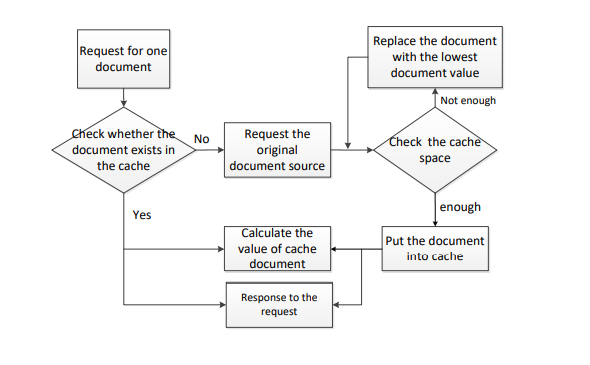
\includegraphics[width = 0.7\linewidth]{flow_chart.png}}
\caption{Caching Process}
\label{fig}
\end{figure}

\section{WGDSF algorithm process}

\begin{figure}[htbp]
\centerline{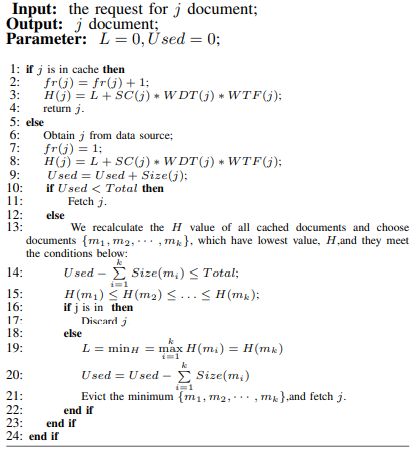
\includegraphics[width = 0.8\linewidth]{code.png}}
\caption{Caching Process}
\label{fig}
\end{figure}

When user request for some document from Cache then\\ (i) if Hit occurred then then we simply update the H-funtion for that particular document and return that document to user.\\
(ii) If miss occurred then we will find the minimal set of documents from our cache which has lower value of H-function. and evect those documents from our cache. This is how our algo works\\ \\ 

\section{Performance Comparison}
We have Compared the proposed algorithm(WGDSF) with FIFO, LRU and GDS alrorithm and found that it has higher hit rate. which is shown below.\\

\begin{figure}[htbp]
\centerline{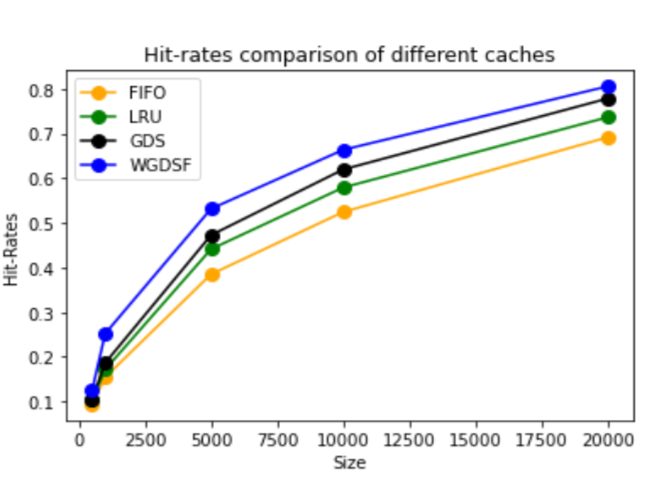
\includegraphics[width = 0.8\linewidth]{testing.png}}
\caption{Comparison with other policies}
\label{fig}
\end{figure}

This algorithm can be put into use in real networks and can get well performance.

\section{Changes which we have implemented}
\subsection{Paging}
Paging was not covered in this proposed algorithm, which we have implemented in our implementation. we found that hit rate decreased as compared to without paging implementation but still it was better than other three replacement policy. results are shown below

\begin{figure}[htbp]
\centerline{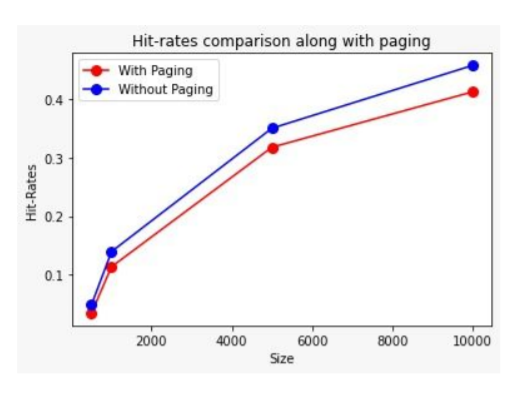
\includegraphics[width = 0.8\linewidth]{paging.png}}
\caption{Comparison of paging and non-paging}
\label{fig}
\end{figure}

\subsection{Change in TCP segment size}
We tried to change the proposed TCP socket size which is predefined as 536 as maximum. We tried to change the value to different varying number.It turns out that the Hit Rate is ambiguous for different socket sizes as the difference is very less.


\begin{figure}[htbp]
\centerline{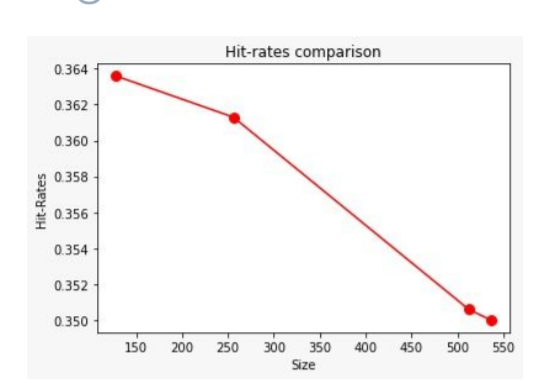
\includegraphics[width = 0.8\linewidth]{tcp.png}}
\caption{}
\label{fig}
\end{figure}

\section{Implementation}

\hyperlink{Source Code : }{https://github.com/sudarshannn/SRI-21}

\section{References}
Weighted Greedy Dual Size Frequency
based Caching Replacement Algorithm 
TINGHUAI MA1,2 (Member, IEEE), JINGJING QU1, WENHAI SHEN3 ,YUAN TIAN4, ABDULLAH AL-DHELAAN3, AND MZNAH AL-RODHAAN4



\end{document}
